{
	\section{Ծրագրային կոդի հատկությունների հարցումների համակարգի իրականացում}\label{sec:queryEngineImplementation}
	Այս բաժնում ներկայացվում է ծրագրային կոդի հատկությունների հարցումների համակարգի իրականացման գործընթացը:
	Այն ներառում է հարցումների ավտոմատ գեներացման համակարգի մշակումը, ծրագրի ներքին կառուցվածքը նկարագրող բաղադրյալ
	գրաֆի կառուցումը, ինչպես նաև տվյալների հոսքի վերլուծությունն ակտիվ փոփոխականների վերլուծությամբ: Այս
	բաժինը ներկայացնում է համակարգի իրականացման հիմնական մոտեցումներն ու մեթոդները՝ արդյունավետ
	և հուսալի հարցումների համակարգ ապահովելու համար:

	{
    \subsection{Հարցումների ավտոմատ գեներացման համակարգ}\label{subsec:queryAggregation}
}

	{
	\subsection{Բաղադրյալ գրաֆ}\label{subsec:proceduregraph}
	Ծրագրային կոդի հատկությունների վերլուծություններն իրականացնելու համար օգտագործվել է բաղադրյալ գրաֆ կառուցվածքը։
	Բաղադրյալ գրաֆն ուղորդված գրաֆ է, որի գագաթները ներկայացնում են միջանկյալ ներկայացման   հրամաններ, ֆունկցիայի պարամետրեր,
	գլոբալ փոփոխականներ, դասի անդամ փոփոխականներ, իսկ կողերը ցույց են տալիս գրաֆի գագաթների միջև ղեկավարման և
	տվյալային կախվածությունները (Նկար \ref{fig:figure8}):

	\begin{figure}[h]
		\centering
		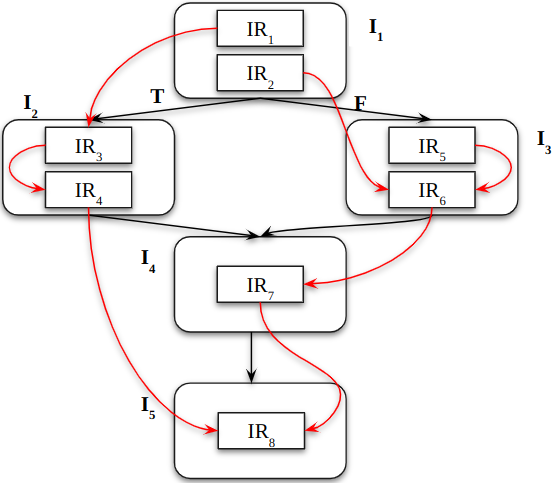
\includegraphics[width=0.7\textwidth]{pic8}
		\caption{Բաղադրյալ գրաֆ}
		\label{fig:figure8}
	\end{figure}

	Բաղադրյալ գրաֆը կառուցվում է ղեկավարման հոսքի գրաֆի հիման վրա, նրան ավելացնելով հավելյալ գագաթներ և կողեր։
	Ավելացվող գագաթներն իրենցից ներկայացնում են այն գլոբալ փոփոխականների կամ դասերի դաշտերի հայտարարումները, որոնից
	գրաֆի գագաթներին համապատախանող հրահանգներում առկա է տվյալային կախվածություն։ Ավելացվող կողերը ցույց են տալիս գրաֆի
	գագաթներին համապատասխանող հրահանգների միջև առկա տվյալային կախվածությունները։

	Ծրագրի հրահանգների փոխարեն, որպես բաղադրյալ գրաֆի գագաթներ են օգտագործվել միջանկյալ ներկայացման հրամանները։
	Այդ կերպ բարձրացվել է կատարվող վերլուծությունների ճշտությունը։  Նկար \ref{fig:figure9}-ում ներկայացված է աղբյուր կոդը
	և այդ կոդի բաղադրյալ գրաֆը։ Ինչպես երևում է բաղադրյալ գրաֆից, ֆունկցիայի կողմից վերադրաձվող v2 փոփոխականի արժեքը
	հաստատուն է և կախված չէ ֆունկցիայի x արգումենտից։

	\begin{figure}[h]
		\centering
		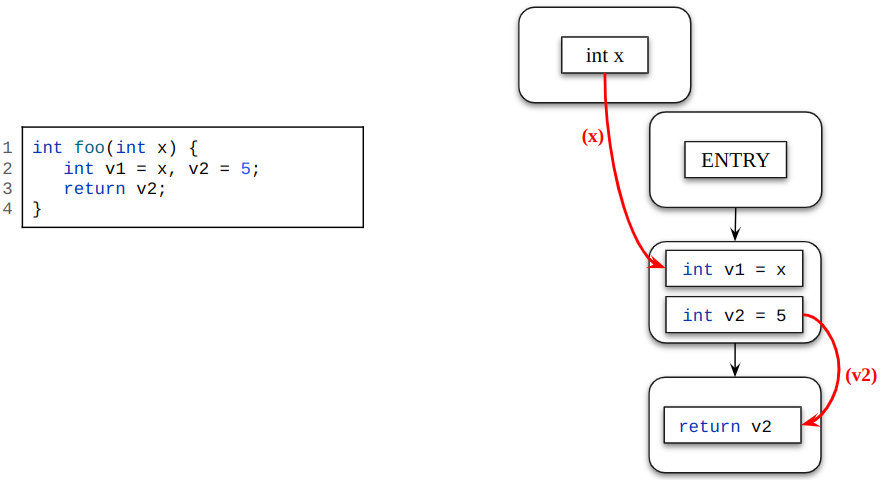
\includegraphics[width=1\textwidth]{pic9}
		\caption{Աղբյուր կոդ օրինակ և համապատասխանող բաղադրյալ գրաֆը}
		\label{fig:figure9}
	\end{figure}

	\subsubsection{Տվյալների հոսքի վերլուծություն}
	
	Տվյալների հոսքի վերլուծությունը ծրագրի կատարման ճանապարհներին տվյալների հոսքերի մասին ինֆորմացիայի հավաքագրումն է։
	Այն կատարվում է ղեկավարման հոսքի գրաֆի հիման վրա։ Տվյալների հոսքի վերլուծության երկու հիմնական մեթոդներն են ակտիվ
	փոփոխակաների և հասնող սահմանումների\cite{aho} վերլուծությունները։ Գործիքում տվյալների հոսքի վերլուծությունը
	կատարվել է  ակտիվ փոփոխականների վերլուծությամբ։
	
	\subsubsection{Ակտիվ փոփոխականների վերլուծություն}
	
	Փոփոխականն ակտիվ է ծրագրի որոշակի կետում, եթե իրեն վերագրված արժեքը ղեկավարման հոսքի գրաֆում իր ժառանգների կողմից օգտագործվում է:
	Վերլուծություն կատարելու համար օգտագործում ենք հետևյալ չորս բազմությունները՝ \textit{def}, \textit{use}, \textit{in} և \textit{out}։
	Ղեկավարման հոսքի V գագաթի def բազմությունը պարունակում է այն փոփոխականները, որոնք արժեքավորվել են V գագաթում,
	իսկ use բազմությունը՝ որոնք օգտագործվել են V գագաթում։ Ունենալով այս երկու բազմությունները, կարող ենք հաշվել in և out
	բազմությունները (այսինքն ակտիվ փոփոխականների բազմությունը գագաթ մուտք գործելիս և գագաթից դուրս գալիս),
	հետևյալ հավասարումների միջոցով\cite{aho}.
	
	{		
		\vspace{-\baselineskip}	
		\begin{align*}
			&\text{IN}[exit] = \varnothing & \\
			&\text{IN}[V] = \text{use}[V] \cup (\text{OUT}[V] \setminus \text{def}[V]) & \\
			&\text{OUT}[V] = \bigcup_{s \in \text{V}{successors}} \text{IN}[s] & 
		\end{align*}
	}

	Նկատենք, որ in և out բազմությունները հաշվելու հավասարումները ռեկուրսիվ են և փոխկապակցված։ Առաջին հավասարումը
	սահմանում է սահմանային պայմանը։ Սա նշանակում է, որ ծրագրի ավարտին ակտիվ փոփոխականներ չկան։ Երկրորդ հավասարումով
	ասվում է, որ փոփոխականը գագաթ մուտք գործելիս ակտիվ է, եթե այն օգտագործվում է գագաթում, կամ դուրս է գալիս գագաթից
	առանց վերասահմանվելու։ Երրորդ հավասարումով ասվում է, որ գագաթից դուրս գալիս փոփոխականն ակտիվ է այն և միայն այն
	դեպքում, երբ այն ակտիվ է իր ժառանգ գագաթներից գոնե մեկում։
	
	\subsubsection{def և use բազմություններ}
	Յուրաքանչյուր գագաթում առկա փոփոխականները դիտարկվում են կամ  որպես սահմանվող(def) կամ որպես օգտագործվող(use)
	փոփոխականներ։ Որոշ  փոփոխականներ դիտարկվում են և որպես սահմանվող, և որպես օգտագործվող փոփոխակներ։ Օրինակ, եթե
	դիտարկենք “++” post increment օպերատորը, “var++” արտահայտությունում var փոփոխականը և օգտագործվում է և նորից
	սահամանվում։ Դիտարկված փոփոխականներն ավելացվում են def և use բազմություններում։

	Այսպիսով կատարվում է def և use փոփոխականների վերլուծություն և ղեկավարման հոսքի գրաֆի յուրաքանչյուր գագաթի համար
	տրվում է այդ գագաթի def և use բազմությունները։ Նկար \ref{fig:figure10}-ում ցուցադրված է Նկար \ref{fig:figure9}-ի
	օրինակին համապատասխանող def և use բազմությունները։

	\begin{figure}[h]
		\centering
		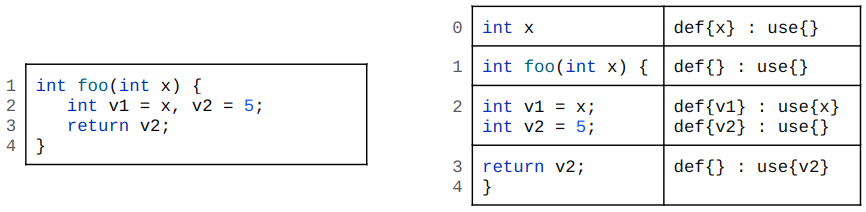
\includegraphics[width=1\textwidth]{pic10}
		\caption{def և use բազմություններ}
		\label{fig:figure10}
	\end{figure}
	
}
}
